\documentclass{article}
\usepackage{kotex}
\usepackage{graphicx}
\usepackage{subfigure}
\usepackage{caption}
\usepackage{fullpage}
\usepackage{amsfonts}

\title{프로그래밍언어_HW0}
\author{유송경}

\begin{document}

\section{자기소개}
이름 : 유송경 \\
학번 : B935277 자율전공학과 (주전공: 컴퓨터공학과)\\
거주 : 서울 \\
MBTI : ESTJ \\



\section{수식 쓰기}
\# 18 평균변화율 \\
 ◆$x$ 의 증분과 $y$ 의 증분
 함수 $f(x)$ 에서 $x$ 의 값이 $a$ 에서 $b$까지 변할 때, 함숫값 $y$ 는 $f(a)$ 에서 $f(b)$ 까지 변한다. \\
 - $x$의 값의 변화량 $b-a$ 를 $x$ 의 증분이라 하고, $\Delta$ $x=b-a$ \\
 - $y$의 값의 변화량 $f(b)-f(a)$ 를 $y$ 의 증분이라 하고, $\Delta$ $y=f(b)-f(a)$ \\ \\
 ◆ 평균변화율\\
 - $x$ 의 증분 $\Delta$$x$에 대한 $y$의 증분 $\Delta$ $y$의 비 \\
 -$\frac{\Delta y}{\Delta x}$=$\frac{{f(b)-f(a)}}{{b-a}}$=$\frac{{f(a+\Delta x)-f(a)}}{\Delta x}$ \\

\newpage

\section{좋아하는 사진}

\label{sec:sec1}
\subsection{자신을 나타낼 수 있는 사진}
\label{sec1:subsec1}
\begin{figure}[h!]
\begin{center}
    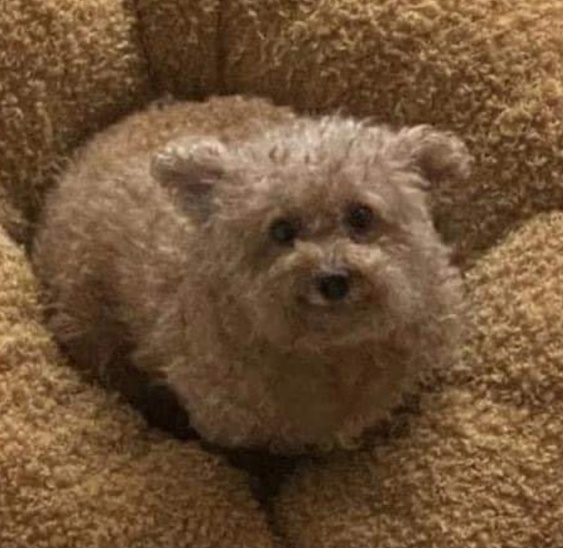
\includegraphics[scale=0.4]{happydoggy.jpg}
    \caption{자신을 나타낼 수 있는 사진}
    \label{fig:fig1}
    \ref{sec1:subsec1} 저와 닮은 강아지 입니다.
\end{center}

\label{sec:sec2}
\subsection{좋아하는 연예인 사진}
\label{sec2:subsec2}
\begin{center}
    \subfigure[생일송강]{
\includegraphics[width=0.4\textwidth]{songgang2.png}}
    \subfigure[스위트홈송강]{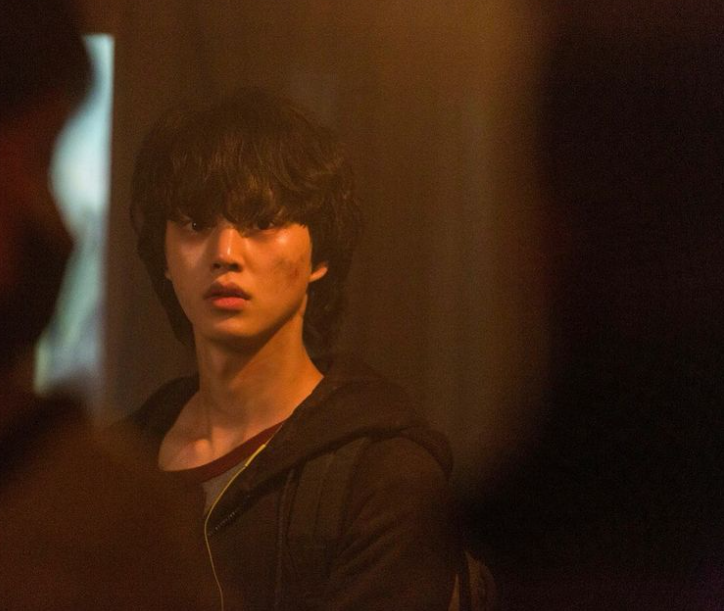
\includegraphics[width=0.5\textwidth]{songgang1.png}}
    \caption{좋아하는 연예인}
    \label{fig:fig2}
    \ref{sec2:subsec2} (a)는 송강의 생일날이고 (b)는 스타트업 촬영장이다.
\end{center}
\end{figure}
\end{document}
